\documentclass{comjnl}

\usepackage{amsmath}
\usepackage{hyperref}
\usepackage{float}
\newcommand*\chem[1]{\ensuremath{\mathrm{#1}}}

%% These two lines are needed to get the correct paper size
%% in TeX Live 2016
%\let\pdfpageheight\paperheight
\let\pdfpagewidth\paperwidth

%\copyrightyear{2009} \vol{00} \issue{0} \DOI{000}

\begin{document}

\title[Superconductivity in Rutherford \texorpdfstring{MgB\textsubscript{2}}{MgB2}  cables and cuprate/manganite multilayer]{How superconductivity in Rutherford \texorpdfstring{MgB\textsubscript{2}}{MgB2}  cables and cuprate/manganite multilayer is affected by external factors}
\author{Even M. Nordhagen}
\affiliation{Computational physics group, Department of Physics, University of Oslo, Oslo, Norway} \email{evenmn@fys.uio.no}

\shortauthors{E. M. Nordhagen}
 
\received{00 November 2017}
\revised{00 Month 2017}


%\category{C.2}{Computer Communication Networks}{Computer Networks}
%\category{C.4}{Performance of Systems}{Analytical Models}
%\category{G.3}{Stochastic Processes}{Queueing Systems}
%\terms{Internet Technologies, E-Commerce}
\keywords{Superconductivity; Rutherford cable; Cuprate; Manganite; YBCO; Transport measurements; Magneto Optical Imaging}


\begin{abstract}
We investigate the superconductive properties of 12-strands twisted Rutherford \texorpdfstring{MgB\textsubscript{2}}{MgB2} cables and a 10-layer \texorpdfstring{Pr\textsubscript{0.5}La\textsubscript{0.2}Ca\textsubscript{0.3}MnO\textsubscript{3}/YBa\textsubscript{2}Cu\textsubscript{3}O\textsubscript{7}}{Pr0.5La0.2Ca0.3MnO3/YBa2Cu3O7} (PLCMO/YBCO) superlattice using transport measurements and magneto-optical imaging, with the former as the main focus. The transport measurements were done carefully, where we studied how the resistance and current through the sample was affected by the temperature. Liquid helium was used to cool down the sample to lower temperatures (min 3.7 K), and for a bit higher temperatures we used liquid nitrogen (min 77 K).  Magneto-optical imaging was most efficient for the Rutherford tape.
\end{abstract}

\maketitle


\section{Introduction}
Since the industrial revolution, humans have burned tremendous amounts of oil to get energy, essentially for electricity or transport usage. Exactly how much oil is remaining on Earth is unknown, and how much we can make use of it depends on the future technology. However, what is sure is that it will not last forever, and we need to find new, preferably renewable, energy sources. What if we could find a renewable energy carrier which was so cold that it could support superconductivity at the same time? We do not need to search further, the solution is liquid hydrogen! When hydrogen reacts with oxygen, we get water, which is 100\% renewable, at the same time as liquid hydrogen has a temperature of 20 K.

To improve the hydrogen economy, we need a material which is superconducting above 20 K and can be made on large scale. For a long time, this material was not avaliable, but in 2001 a group of Japanese scientists found that \chem{MgB_2} has transition temperature of \chem{T_c} = 39 K, which is one of the highest in conventionable superconductors \cite {jsap}\cite {nature}. This again gave hope for possible large-scale applications of superconductors using cryogen-free technology. 

We are going to study a Rutherford cable consisting of strands with cores of \chem{MgB_2}. Rutherford cables are frequently used to generate magnetic fields in particle accelerators, and were first developed at the Rutherford Laboratory, hence the name \cite {fnal}. Our sample was sent from Spain, and we will return the results as soon as they are ready. Maybe we participate in developing the next generation particle accelerators?

Moreover we have examined the superconducting properties of a YBCO multilayer sample. YBCO has status as the first material to be found superconducting above the temperature of liquid nitrogen, which generated major optimism for superconductivity when it was discovered in 1987 \cite{harvard}, with its critical temperature of \chem{T_c} = 92 K. 

\section{Theory}\label{Sec:Theory}
Superconducting materials have two main properties: they are resistance-free conductors below critical temperature \chem{T_c} and magnetic field cannot penetrate the material below the same temperature \chem{T_c}. The methods we use are based on both these main properties. Perhaps the easiest way to find the resistance of a sample is to connect the sample to a power supply and measure the voltage difference, U, between two points. The resistance can then be calculated by Ohm's law U = RI, given the current I. This is known as a four-point measurement or four-terminal sensing, and is widely used in transport measurements. No voltage drop corresponds to zero resistance. In figure (\ref{fig:4point}) one can find a sketch of a four-point measurement. It is crucial that all the contacts are made all the way across the sample, such that the current is uniformly distributed. It should neither be able to avoid the potential contacts.
\begin{figure}[h]
\centering
\includegraphics[width=70mm]{4point.png}
\caption{General 4-point method with four contacts. The two outermost (I1 and I2) are connected to current cables, such that current flows through the sample, while the innermost contacts (U1 and U2) are connected to potential wires. See text for further reading. \label{fig:4point}}
\end{figure}

In some cases it is appropriate to use more advanced techniques, for instance when the sample structure is not uniform in every direction. Then we might want to measure the resistance in various directions, but without disturbing the samples with more contacts than necessary. By placing the contacts in each corner, we can reuse the contacts when "turning" the sample, known as the Montgomery technique, illustrated in figure (\ref{fig:4corner}). 

\begin{figure}[h]
\centering
\includegraphics[width=60mm]{4corner.png}
\caption{The 4-corner measurement is used in the Montgomery technique to study the anisotropy of a sample. Contact U1 and U2 are connected to a voltmeter, while contact I1 and I2 are the current contacts. \label{fig:4corner}}
\end{figure}

\subsection{Magneto-Optical Imaging (MOI)}
Our eyes are not able to see magnetism, but with a MOI apparatus we can take pictures of a magnet or superconductor and decide if a sample is superconducting, using the elementary magnetic property discussed in section \ref{Sec:Theory}. The method is quite simple where light is reflected by a Faraday crystal on top of the sample. If the Faraday crystal is affected by a magnetic field, it will polarize the light, and it will later be separated out by a polarization filter, as shown in figure (\ref{fig:MOI}). The idea is that all the light will not go through the filter as long as the sample is not superconducting. Alternatively if the sample is superconducting, we will get light passing outside superconducting area. Not only can MOI detect superconductivity, but we can also see exactly where the material is superconducting, which is convenient for non-homogeneous materials. 
\begin{figure}[h]
\centering
\includegraphics[width=80mm]{moi.png}
\caption{A simple sketch of a MOI apparatus, which consists of two polarizators, a couple of mirrors, a magnet, a Faraday crystal and a photo detector. See text to find out how it works. \label{fig:MOI}}
\end{figure}

\section{Experiments}\label{Sec:Experiments}
Now as the theory is introduced, we are ready to see how the experiments actually were done. Our samples are the Rutherford tape consisting of 12 strands and the YBCO multilayer. Only the former gives good results in Magneto-Optical imaging, while we did transport measurements on both. 

\subsection{Rutherford tape}
A Rutherford cable is a cable consisting of multiple layers of different materials. Our sample has a core of superconducting \chem{MgB_2} (with 39 K as the transition temperature) covered by a layer of Niobium, which is another superconductor with critical temperature 9.2 K. We then expect really low total resistance below 9.2 K, a little more resistance between 9.2 K and 39 K, and no superconductivity above 39 K. The niobium layer is again covered by the non-superconducting metal \chem{Cu_{10}Ni}, to protect the cable. A cross-section optical image is shown in figure (\ref{fig:rutherford2}).
\begin{figure}[h]
\centering
\includegraphics[width=50mm]{rutherford2.jpg}
\caption{Cross-section of the Rutherford cable, showing the \chem{MgB_2} core (dark) apparently covered by a gray layer. Both the outermost layers look gray and it is hard to differ them on an optical image. The picture was taken after polishing, as we can see its effect on some of the wires. \label{fig:rutherford2}}
\end{figure}

\subsubsection{Transport Measurements}
The transport measurements on the Rutherford tape were done using 4-point connection defined in the theory. We used liquid helium to cool down the sample, because liquid nitrogen would not be cold enough. First we placed the sample on the sample holder, and connected current and potential contacts. The contacts were made of indium (In) since it is a good conductor and easy to apply, see figure (\ref{fig:sampleholder}) for a picture after the cables are connected. Then we had to attach the sample to the rod using adhensive tape. This tape worked as an isolator for the potential and current cables at the same time. To ensure the tape would not loosen, we strapped a thread around it. 

\begin{figure}[h]
\centering
\includegraphics[width=70mm]{sampleholder.jpg}
\caption{The Rutherford tape placed on sample holder where all the four cables are connected.  \label{fig:sampleholder}}
\end{figure}

Further we added heat isolation to make the temperature changes more smooth. First a finger was cut of a blue vinyl glove, and attached around the sample with tape. Unfortunately we found this to be too well isolated, so we tried with a transparent finger. This worked better, but the temperature changes were not always as smooth as desired. A vinyl finger would also protect the sample in case it was dipped in the liquid helium. Moreover we struggled with several other isolation mechanisms, they were not always successful. 

After the sample holder was prepared, we could measure the resistance as the sample was dipped into the liquid helium container. We measured both on the way down and on the way up, and sometimes we went up and down around critical temperature to see if we got hysteresis and how eventually big it was. In section \ref{Sec:Results} the results are presented.

\subsubsection{Magneto-Optical Imaging (MOI)}
Before the MOI analysis was done, we polished the sample to get the Faraday crystal closer to the superconducting part. This was done by a rotating sandpaper, and an image of polished sample is shown in figure (\ref{fig:rutherford1}). Thereafter we cleaned it and placed it on the sample holder using vacuum grease which becomes sticky in vacuum. The Faraday crystal can not be attached to the sample in any way, so we need restrictions to make sure that it did not fall of the sample. When the sample was prepared, we could go further and prepare for the experiment. We placed sample holder with sample inside MOI cryostat and made vacuum (pressure below 1E-4 mBar), and finally we cooled down the system using liquid helium.
\begin{figure}[h]
\centering
\includegraphics[width=70mm]{rutherford1.jpg}
\caption{This is how the Rutherford tape looked after polishing. If one looks carefully, it is not uniformly polished. Especially the lower part is not ideal. \label{fig:rutherford1}}
\end{figure}
\begin{figure}[h]
\centering
\includegraphics[width=50mm]{sampleholder2.jpg}
\caption{Rutherford cable placed on the MOI sample holder, covered by a Faraday crystal. A watchful eye will see the restrictions to keep the Faraday crystal on top. \label{fig:sampleholder2}}
\end{figure}

\subsection{PLCMO/YBCO multilayer}
We have a sample consisting of 10 extremely thin layers of \chem{YBa_2Cu_3O_7} (YBCO) with \chem{Pr_{0.5}La_{0.2}Ca_{0.3}MnO_3} (PLCMO) in-between. YBCO is superconducting at 92 K, and we can therefore study the superconducting properties even in liquid nitrogen. PLCMO is not a superconductor, and with thickness 20 nm it is thicker than the YBCO layers, which are 7 nm each. 

\subsubsection{Transport measurements}
For this sample the transport measurements were conducted using the 4-corner configuration, which makes us able to study the anisotropy. In figure (\ref{fig:multilayer}) one see how wires were connected to the sample.
\begin{figure}[h]
\centering
\includegraphics[width=60mm]{multilayer.png}
\caption{The cables are connected to the YBCO multilayer using the 4-corner connections. \label{fig:multilayer}}
\end{figure}
We later turned the sample, i.e, all the cables were connected to the neighbor contacts and we repeated the measurements, referred to as the Montgomery technique. 

First we investigated the superconductiving properties of wires at low temperature using liquid helium as the cooling medium, but after a few days with measurements we ran out of liquid helium and had to use liquid nitrogen. When using liquid helium, the container was equiped with a holder, which made it easy to dip the sample into the helium slowly and lift it carefully. We did not have this equipment for the liquid nitrogen container, and had to develop our own construction. An image of this construction in use is shown in figure (\ref{fig:patent}). The sample was dipped into a pot containing liquid nitrogen as showed in figure (\ref{fig:nitrogen}). 
\begin{figure}[h]
\centering
\includegraphics[width=60mm]{patent.jpg}
\caption{Our own contruction was able to increase and decrease the rod with the sample smoothly. On the floor one can spot the pot with liquid nitrogen. \label{fig:patent}}
\end{figure}
\begin{figure}[h]
\centering
\includegraphics[width=40mm]{nitrogen.jpg}
\caption{Pot with liquid nitrogen. \label{fig:nitrogen}}
\end{figure}
Also for this sample we did measurements both on the way down and on the way up in temperature, but our construction made it difficult to lift the sample such that the temperature change was constant. Instead of moving it slowly upwards, we laid the cooled sample on a table and measured when it approached room temperature. To keep smooth temperature changes, it was pushed into a thick, isolating glove, as shown in figure (\ref{fig:glove}).
\begin{figure}[h]
\centering
\includegraphics[width=40mm]{glow.jpg}
\caption{A thick glove was used to heat the sample slowly. \label{fig:glove}}
\end{figure}


\section{Results}\label{Sec:Results}
As section \ref{Sec:Experiments} indicates, we have studied Rutherford cable by transport measurements with a 4-point connection, and also magneto-optical imaging has been used to reveal the superconducting properties of the sample. Additionally the YBCO multilayer has been investigated by transport measurements using the 4-corner connection. The experiments are detailed in section \ref{Sec:Experiments}.

\subsection{Rutherford cable}
\subsubsection{Transport measurements}
All the transport measurements were done using liquid helium as cooling medium. In figures (\ref{fig:rutherfordRTallI}) and (\ref{fig:rutherfordRTlowI}) one can find resistance plotted as function of temperature for low currents in the temperature range 160 K to 25 K and around the critical temperature, respectively. 
\begin{figure}[h]
\centering
\includegraphics[width=70mm]{Rutherford_RT_all_T_low_I.png}
\caption{Resistance plotted as function of temperature from 160 K to 25 K. The dark graph is 0.2 A, the blue graph is 0.5 A and the pink graph is 0.7 A. \label{fig:rutherfordRTallI}}
\end{figure}
\begin{figure}[h]
\centering
\includegraphics[width=70mm]{Rutherford_RT_low_I.png}
\caption{Resistance plotted as a function of temperature around the critical temperature. The dark graph is for 0.2 A, the blue graph is for 0.5 A and the pink graph is for 0.7 A. \label{fig:rutherfordRTlowI}}
\end{figure}
As one can see in figure (\ref{fig:rutherfordRTallI}), all the curves seem to follow almost the same path, but with more spread for higher temperatures. We get transition of 37 K, as expected, and on the zoomed-in plot in figure (\ref{fig:rutherfordRTlowI}) one can see that we got trasition for the highest temperature at 0.5 A, followed by 0.7 A and 0.2 A. This is suspicious since higher currents should give us transition at lower temperature. Furthermore we study the hysteresis in figure (\ref{fig:rutherfordRT}), where resistance is plotted against the temperature for 0.05 A, 0.1 A and 0.3 A. We can immediately see that the graphs are ordered correctly in this plot, with 0.05 A as the graph with transistion at highest temperature.
\begin{figure}[h]
\centering
\includegraphics[width=70mm]{Rutherford_RT.png}
\caption{Resistance as a function of temperature around the critical temperature. The red graph corresponds to 0.05 A, the black corresponds to 0.1 A and the blue one corresponds to 0.3 A. See text for futher description. \label{fig:rutherfordRT}}
\end{figure}


\subsubsection{Magneto-optical imaging}
We did magneto-optical imaging as described in section \ref{Sec:Experiments}, and we got the image presented in figure (\ref{fig:moi2d1}) when a current of 3.4 A was sent through the coil of magnet. Unlike for the optical image, we can now clearly see the different layers, where the brighter area is \chem{MgB_2}, the dark layer covering the core is Niobium and the outermost layer is \chem{Cu_{10}Ni}. We can also spot a darker line in the \chem{Cu_{10}Ni}, which is the gap between two different wires of strands. In section (\ref{Sec:Theory}) it was stated that the light should not be polarized in the area where we had superconductivity, and the magneto-optical image should therefore have dark areas where the sample is superconducting. In this figure (\ref{fig:moi2d1}) it is opposite, and the reason is that the image is negative. 
\begin{figure}[h]
\centering
\includegraphics[width=80mm]{scale_no_79_d_I_3p4_V_0p6_A.png}
\caption{MOI analyse of the Rutherford cable, where the current in magnetic coil was 3.4 A and the temperature was 3.7 K. The length of the scale bar is 0.1mm. \label{fig:moi2d1}}
\end{figure}

Furthermore, we did the same experiment, but with no current in the coil with another polarization and with an 2.5x optical objective instead of 10x. The result is presented in figure (\ref{fig:moi2d2}). 
\begin{figure}[h]
\centering
\includegraphics[width=80mm]{scale_no_119_obj_2p5_pol_m3_grey.png}
\caption{MOI image of the Rutherford cable with no current flowing in the coil at temperature of 3.7K and polarization angle of 2.5 degrees. The scale bar has length 1 mm. \label{fig:moi2d2}}
\end{figure}

We also played with a 3D tool to transform a 2D magneto-optical image into a 3D image where the z-axis showed the intensity of polarization. As we can see in figure (\ref{fig:moi3d}), all of the sample apart from the outermost layer is superconducting at 3.7 K. Again we can spot the gap between the strands, which appears as red spikes in the non-superconducting area. 
\begin{figure}[h]
\centering
\includegraphics[width=80mm]{3D_Diff_no_85_i_I_m1p0_V_m0p2_A_m0p4_A_sc.png}
\caption{Color coded MOI image of the Rutherford cable with current in the coil of 1.0 A and temperature of 3.7 K. The scale bar has length of 0.1 mm. The level along z-axis indicates where the sample is superconducting.\label{fig:moi3d}}
\end{figure}

\subsection{YBCO}
\subsubsection{Transport measurements}
In figure (\ref{fig:res_norm}), the resistance is plotted as function of the temperature for currents from 4.3 mA to 37.0 mA, where the current flows parallel to the defect. We observe that the initial resistance is approximately the same, no matter what the current is, but when cooling down, the resistance drops stronger for low currents and is more constant for higher currents. 
\begin{figure}[h]
\centering
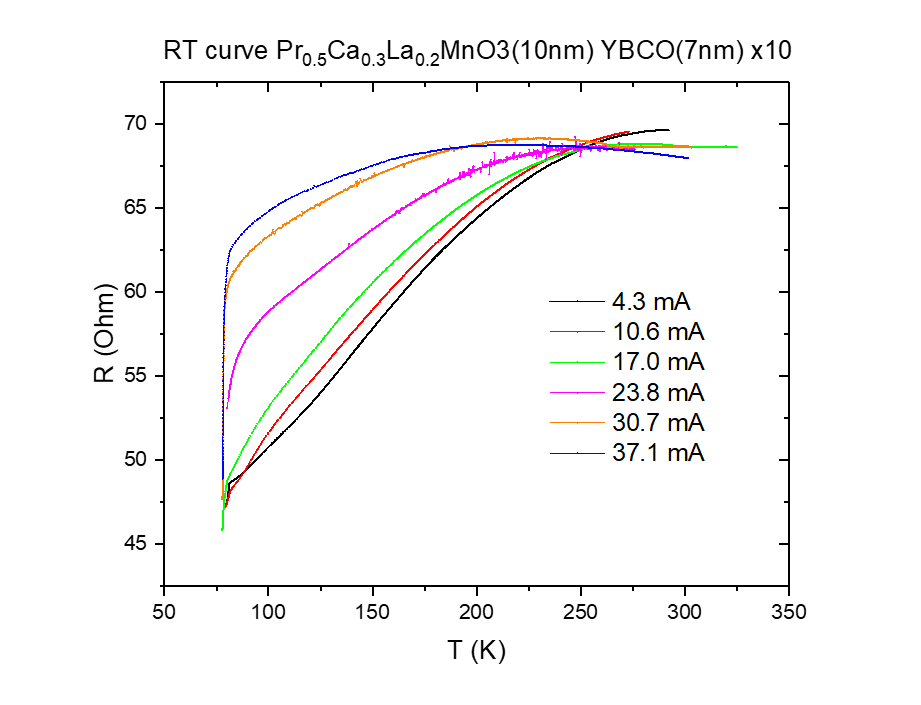
\includegraphics[width=100mm]{Bilde1.png}
\caption{Resistance as function of temperature from 298 K (room temperature) to 80 K with liquid nitrogen as the cooling medium. The black graph is the graph at current 4.3 mA, the red graph corresponds to 10.6 mA, the green graph to 17.0 mA, the magenta to 23.8 mA, the orange to 30.7 mA and finally the blue one to 37.0 mA. \label{fig:res_norm}}
\end{figure}
Further we used the Montgomery technique to turn the sample, and observed the resistance with current flowing perpendicular to the defect, with the result plotted in figure (\ref{fig:res}). As we can see, the initial resistance is higher when the current flows perpendicular to the defect than parallel to it. 
\begin{figure}[h]
\centering
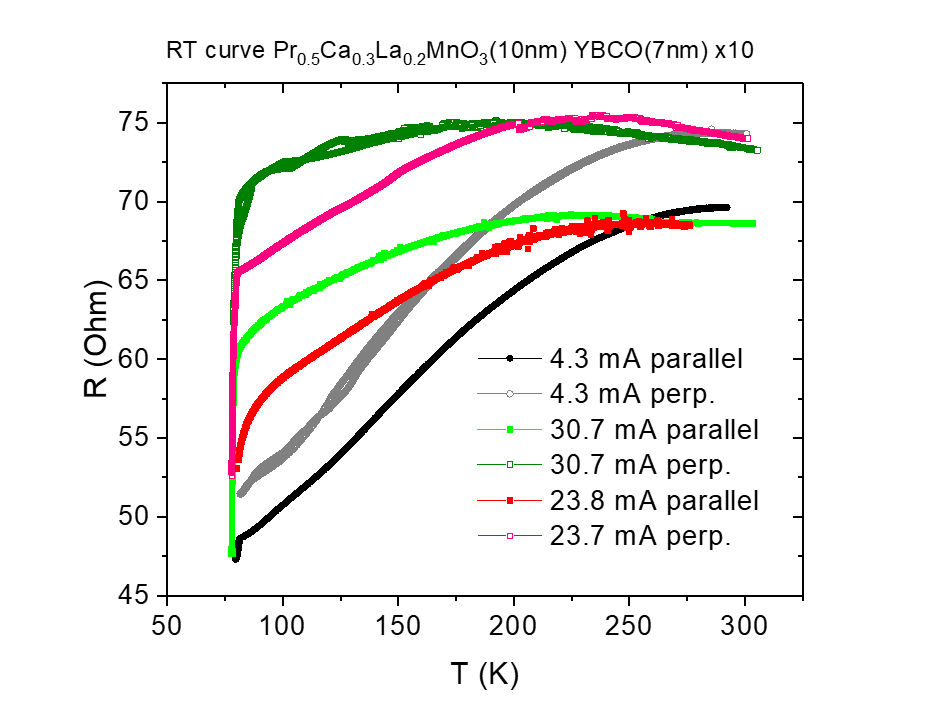
\includegraphics[width=100mm]{Bilde2.png}
\caption{In this plot we compare the resistance of the parallel case with the perpendicular case, and plot them as functions of temperature from 298 K (room temperature) to 80 K with liquid nitrogen as the cooling medium. The black, red and lime colored graphs correspond to 4.3 mA, 23.8 mA and 30.7 mA for the parallel case, respectively, while the gray, magenta and olive colored graphs correspond to 4.3 mA, 23.7 mA and 30.7 mA, respectively, for the perpendicular case. \label{fig:res}}
\end{figure}

Moreover, we studied how the current was changing as the temperature decreased for both the parallel and perpendicular case, and the result is shown in figure (\ref{fig:cur}). The legend indicates the initial current. We see that the currents are roughly the same in both cases, so it is enough to study one of them, but whereas the two higher currents increase for low temperatures, the lower current seems to decrease. It would therefore be interesting to see how the current graphs are behaving when we normalize them, and a plot of that is presented in figure (\ref{fig:cur_norm}). 
\begin{figure}[h]
\centering
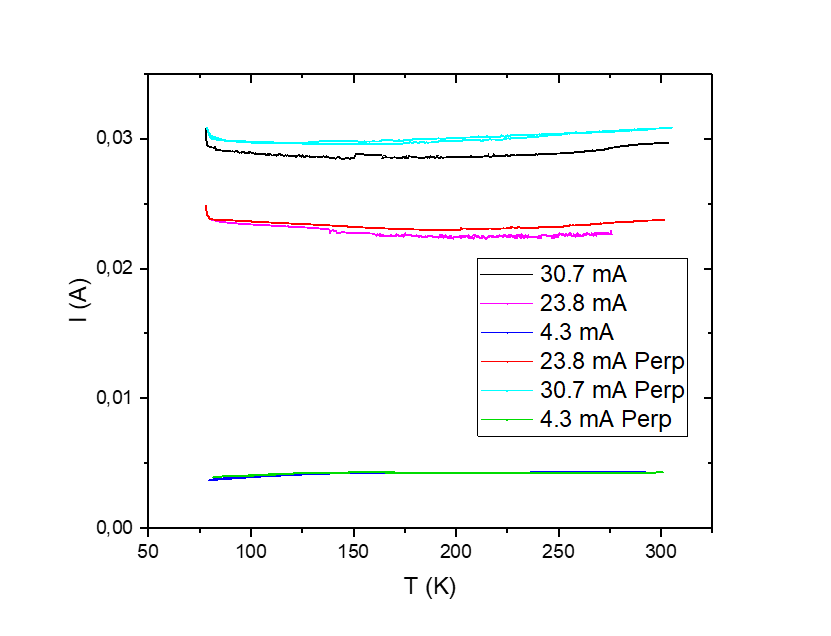
\includegraphics[width=100mm]{Bilde3.png}
\caption{The current as a function of temperature with 4.3 mA, 23.7 mA and 30.7 mA as initial currents for both current flowing parallel and perpendicular to the defect.\label{fig:cur}}
\end{figure}
\begin{figure}[h]
\centering
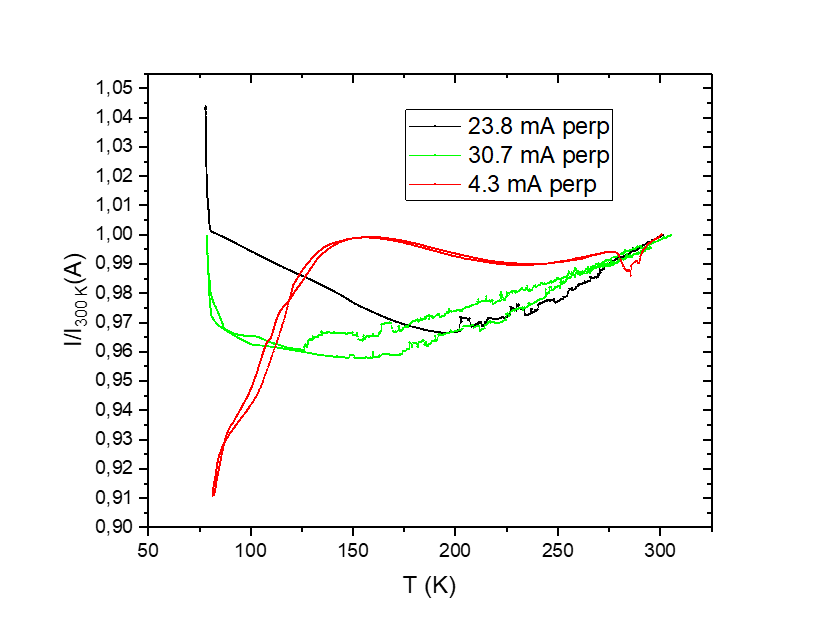
\includegraphics[width=100mm]{Bilde4.png}
\caption{The current as function of temperature with 4.3 mA, 23.7 mA and 30.7 mA as initial currents for the perpendicular case. The currents are normalized with respect to the initial current.\label{fig:cur_norm}}
\end{figure}
As we can see, the lower-current line is actually decreasing at low temperatures, which makes no sense according to Ohm's law. The reason is discussed in section \ref{Sec:Discussion}.

\section{Discussion} \label{Sec:Discussion}
In figures (\ref{fig:rutherfordRTallI}) and (\ref{fig:rutherfordRTlowI}) we got transition at higher temperature when we had I = 0.7 A than T = 0.2 A, which makes no sense. The reason is not clear, but it could be that we increased the temperature too fast, or maybe we got an unusual hysteresis. We have a small distance between the temperature sensor and the sample, which causes some delay in temperature signal provided by sensor, i.e, the temperature from the sensor is slightly different from the actual temperature on the sample. Anyway, in figure (\ref{fig:rutherfordRT}) the curves behave as expected. 

Furthermore, in figure (\ref{fig:moi2d1}) we saw that \chem{MgB_2} was superconducting at 3.7 K, but surprisingly Niobium is dark and indicates that it is not superconducting, which is strange. Maybe the temperature is wrong. Moreover, in figure (\ref{fig:moi2d2}) the sample looks superconducting on the edges of the \chem{MgB_2} core. The reason is that the magnetic field has penetrated the core from both sides. 

In figure (\ref{fig:res}), the resistance was apparently higher when the current flowed perpendicular to the defect, than when it flowed parallel to the defect. This is probably because the contacts are more resistive in this case. Ideally (with the same contacts) the resistance should be the same. Therefore, it would be better to normalize all graphs with respect to the initial resistance to make the comparison easier. We also saw that the higher currents lead to higher resistance for lower temperatures, which causes a big drop when the critial temperature is reached. This is probably because the electrons are not fully spin-polarized, even though the Curie temperature is reached. 

When studying the current as a function of temperature in figures (\ref{fig:cur}) and (\ref{fig:cur_norm}), we found the higher currents to increase rapidly around transition, which is expected since the resistance is dropping. Anyway, for initial current 4.3 mA, the current dropped at low temperatures, which immediately seems strange. The current is affected by the contacts, and since low currents are more sensitive to resistance of contacts, we would probably have gotten the expected result with ideal contacts. 

\section{Conclusion} \label{Sec:Conclusion}
All the time scientists are searching for new knowledge, which is obtained by investigating new materials or new techniques and looking for unusual behavior. This is what we did, but every time we observed something unusual, we were able to explain it using the existing theory. The conclusion is that we did not observe anything fundamental new, but at the same time we managed to investigate a couple of samples, and the information we obtained might be useful for the people who sent us the samples. 

Seen from my perspective, the weeks in the superconductor lab have been very exciting, and it is interesting to see how real scientists are working. Superconductivity is a subject that is fascinating and mind-blowing at the same time, and it has been a pleasure working with it.

\section{References}
\begingroup
\renewcommand{\section}[2]{}
\begin{thebibliography}{}
\bibitem{jsap}
  Discovery of the new superconductor \chem{MgB_2} and its recent development. 
  Y. Zenitani, J. Akimitsu. 
  JSAP International No.6 (July 2002)
  \url{https://www.jsap.or.jp/jsapi/Pdf/Number06/04_CuttingEdge1.pdf}
\bibitem{nature}
  Superconductivity at 39 K in magnesium diboride. 
  J. Nagamatsu, N. Nakagawa, T. Muranaka, Y. Zenitani, J. Akimitsu. 
  Nature 410, 63–64 (01 March 2001)
  \url{https://www.nature.com/articles/35065039}
\bibitem{fnal}
  Development of Rutherford-type Cables for High Field Accelerator Magnets at Fermilab.
  N. Andreev, E. Barzi, E. Borissov, L. Elementi, V.S. Kashikhin, V. Lombardo, A. Rusy, D. Turrioni, 
R.Yamada, A.V. Zlobin.
   Fermi  National  Accelerator  Laboratory,  Batavia, IL 60510 USA (28 August 2016)
  \url{http://lss.fnal.gov/archive/2006/conf/fermilab-conf-06-323-td.pdf}
\bibitem{harvard}
  Superconductivity at 93 K in a new mixed-phase Y-Ba-Cu-O compound system at ambient pressure.
  Wu, M. K.; Ashburn, J. R.; Torng, C. J.; Hor, P. H.; Meng, R. L.
  Physical Review Letters (ISSN 0031-9007), vol. 58, (2 March 1987), p. 908-910.
  \url{http://adsabs.harvard.edu/abs/1987PhRvL..58..908W}
\end{thebibliography}
\endgroup
\nocite{*}

\bibliographystyle{compj}
\bibliography{ModellingBidders}


\end{document}